\documentclass{standalone}
\usepackage{tikz}
\usetikzlibrary{patterns, positioning}

\begin{document}
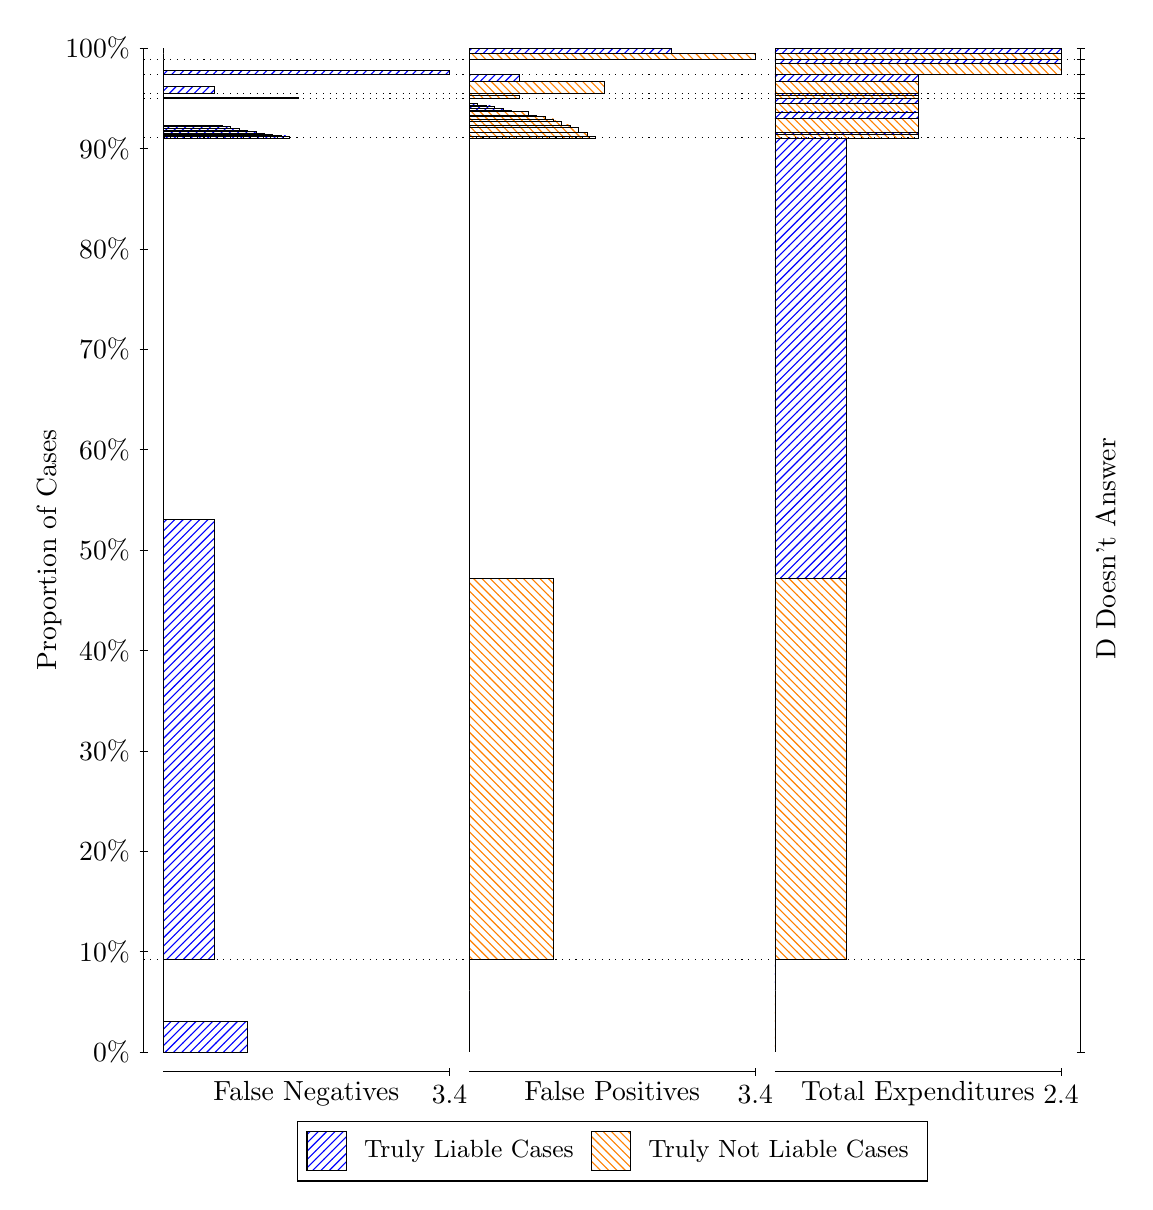
\begin{tikzpicture}
\draw[black, very thin] (1.5,1.75) -- (1.5,14.5);
\node[rotate=90, anchor=center] at (0.3, 8.125) {Proportion of Cases};
\draw[black, very thin] (1.45,1.75) -- (1.55,1.75);
\node[anchor=east] at (1.45, 1.75) {0\%};
\draw[black, very thin] (1.45,3.025) -- (1.55,3.025);
\node[anchor=east] at (1.45, 3.025) {10\%};
\draw[black, very thin] (1.45,4.3) -- (1.55,4.3);
\node[anchor=east] at (1.45, 4.3) {20\%};
\draw[black, very thin] (1.45,5.575) -- (1.55,5.575);
\node[anchor=east] at (1.45, 5.575) {30\%};
\draw[black, very thin] (1.45,6.85) -- (1.55,6.85);
\node[anchor=east] at (1.45, 6.85) {40\%};
\draw[black, very thin] (1.45,8.125) -- (1.55,8.125);
\node[anchor=east] at (1.45, 8.125) {50\%};
\draw[black, very thin] (1.45,9.4) -- (1.55,9.4);
\node[anchor=east] at (1.45, 9.4) {60\%};
\draw[black, very thin] (1.45,10.675) -- (1.55,10.675);
\node[anchor=east] at (1.45, 10.675) {70\%};
\draw[black, very thin] (1.45,11.95) -- (1.55,11.95);
\node[anchor=east] at (1.45, 11.95) {80\%};
\draw[black, very thin] (1.45,13.225) -- (1.55,13.225);
\node[anchor=east] at (1.45, 13.225) {90\%};
\draw[black, very thin] (1.45,14.5) -- (1.55,14.5);
\node[anchor=east] at (1.45, 14.5) {100\%};

\draw[black, very thin] (13.4,1.75) -- (13.4,14.5);
\draw[black, very thin] (13.35,1.75) -- (13.45,1.75);
\node[anchor=west] at (13.35, 1.75) {};
\draw[black, very thin] (13.35,2.9222) -- (13.45,2.9222);
\node[anchor=west] at (13.35, 2.9222) {};
\draw[black, very thin] (13.35,13.359) -- (13.45,13.359);
\node[anchor=west] at (13.35, 13.359) {};
\draw[black, very thin] (13.35,13.856) -- (13.45,13.856);
\node[anchor=west] at (13.35, 13.856) {};
\draw[black, very thin] (13.35,13.922) -- (13.45,13.922);
\node[anchor=west] at (13.35, 13.922) {};
\draw[black, very thin] (13.35,14.169) -- (13.45,14.169);
\node[anchor=west] at (13.35, 14.169) {};
\draw[black, very thin] (13.35,14.357) -- (13.45,14.357);
\node[anchor=west] at (13.35, 14.357) {};
\draw[black, very thin] (13.35,14.5) -- (13.45,14.5);
\node[anchor=west] at (13.35, 14.5) {};

\draw[black, very thin, pattern color=blue, pattern=north east lines] (1.75,1.75) rectangle (2.8186,2.1383);
\draw[black, very thin, pattern color=orange, pattern=north west lines] (1.75,2.1383) rectangle (1.75,2.9222);
\draw[black, very thin, pattern color=blue, pattern=north east lines] (1.75,2.9222) rectangle (2.3912,8.5148);
\draw[black, very thin, pattern color=orange, pattern=north west lines] (1.75,8.5148) rectangle (1.75,13.359);
\draw[black, very thin, pattern color=blue, pattern=north east lines] (1.75,13.359) rectangle (3.3529,13.384);
\draw[black, very thin, pattern color=blue, pattern=north east lines] (1.75,13.384) rectangle (3.2461,13.395);
\draw[black, very thin, pattern color=blue, pattern=north east lines] (1.75,13.395) rectangle (3.1392,13.407);
\draw[black, very thin, pattern color=blue, pattern=north east lines] (1.75,13.407) rectangle (3.0324,13.42);
\draw[black, very thin, pattern color=blue, pattern=north east lines] (1.75,13.42) rectangle (2.9255,13.44);
\draw[black, very thin, pattern color=blue, pattern=north east lines] (1.75,13.44) rectangle (2.8186,13.45);
\draw[black, very thin, pattern color=blue, pattern=north east lines] (1.75,13.45) rectangle (2.7118,13.482);
\draw[black, very thin, pattern color=blue, pattern=north east lines] (1.75,13.482) rectangle (2.6049,13.506);
\draw[black, very thin, pattern color=blue, pattern=north east lines] (1.75,13.506) rectangle (2.498,13.522);
\draw[black, very thin, pattern color=orange, pattern=north west lines] (1.75,13.522) rectangle (1.75,13.856);
\draw[black, very thin, pattern color=blue, pattern=north east lines] (1.75,13.856) rectangle (3.4598,13.874);
\draw[black, very thin, pattern color=orange, pattern=north west lines] (1.75,13.874) rectangle (1.75,13.922);
\draw[black, very thin, pattern color=blue, pattern=north east lines] (1.75,13.922) rectangle (2.3912,14.015);
\draw[black, very thin, pattern color=orange, pattern=north west lines] (1.75,14.015) rectangle (1.75,14.169);
\draw[black, very thin, pattern color=blue, pattern=north east lines] (1.75,14.169) rectangle (5.3833,14.218);
\draw[black, very thin, pattern color=orange, pattern=north west lines] (1.75,14.218) rectangle (1.75,14.357);
\draw[black, very thin, pattern color=orange, pattern=north west lines] (1.75,14.357) rectangle (1.75,14.428);
\draw[black, very thin, pattern color=blue, pattern=north east lines] (1.75,14.428) rectangle (1.75,14.5);
\draw[black, very thin, pattern color=orange, pattern=north west lines] (5.6333,1.75) rectangle (5.6333,2.5339);
\draw[black, very thin, pattern color=blue, pattern=north east lines] (5.6333,2.5339) rectangle (5.6333,2.9222);
\draw[black, very thin, pattern color=orange, pattern=north west lines] (5.6333,2.9222) rectangle (6.702,7.7668);
\draw[black, very thin, pattern color=blue, pattern=north east lines] (5.6333,7.7668) rectangle (5.6333,13.359);
\draw[black, very thin, pattern color=orange, pattern=north west lines] (5.6333,13.359) rectangle (7.2363,13.381);
\draw[black, very thin, pattern color=orange, pattern=north west lines] (5.6333,13.381) rectangle (7.1294,13.424);
\draw[black, very thin, pattern color=orange, pattern=north west lines] (5.6333,13.424) rectangle (7.0225,13.491);
\draw[black, very thin, pattern color=orange, pattern=north west lines] (5.6333,13.491) rectangle (6.9157,13.523);
\draw[black, very thin, pattern color=orange, pattern=north west lines] (5.6333,13.523) rectangle (6.8088,13.574);
\draw[black, very thin, pattern color=orange, pattern=north west lines] (5.6333,13.574) rectangle (6.702,13.601);
\draw[black, very thin, pattern color=orange, pattern=north west lines] (5.6333,13.601) rectangle (6.5951,13.628);
\draw[black, very thin, pattern color=orange, pattern=north west lines] (5.6333,13.628) rectangle (6.4882,13.648);
\draw[black, very thin, pattern color=orange, pattern=north west lines] (5.6333,13.648) rectangle (6.3814,13.694);
\draw[black, very thin, pattern color=blue, pattern=north east lines] (5.6333,13.694) rectangle (6.1676,13.71);
\draw[black, very thin, pattern color=blue, pattern=north east lines] (5.6333,13.71) rectangle (6.0608,13.734);
\draw[black, very thin, pattern color=blue, pattern=north east lines] (5.6333,13.734) rectangle (5.9539,13.766);
\draw[black, very thin, pattern color=blue, pattern=north east lines] (5.6333,13.766) rectangle (5.8471,13.776);
\draw[black, very thin, pattern color=blue, pattern=north east lines] (5.6333,13.776) rectangle (5.7402,13.796);
\draw[black, very thin, pattern color=blue, pattern=north east lines] (5.6333,13.796) rectangle (5.6333,13.856);
\draw[black, very thin, pattern color=orange, pattern=north west lines] (5.6333,13.856) rectangle (6.2745,13.904);
\draw[black, very thin, pattern color=blue, pattern=north east lines] (5.6333,13.904) rectangle (5.6333,13.922);
\draw[black, very thin, pattern color=orange, pattern=north west lines] (5.6333,13.922) rectangle (7.3431,14.076);
\draw[black, very thin, pattern color=blue, pattern=north east lines] (5.6333,14.076) rectangle (6.2745,14.169);
\draw[black, very thin, pattern color=orange, pattern=north west lines] (5.6333,14.169) rectangle (5.6333,14.308);
\draw[black, very thin, pattern color=blue, pattern=north east lines] (5.6333,14.308) rectangle (5.6333,14.357);
\draw[black, very thin, pattern color=orange, pattern=north west lines] (5.6333,14.357) rectangle (9.2667,14.428);
\draw[black, very thin, pattern color=blue, pattern=north east lines] (5.6333,14.428) rectangle (8.198,14.5);
\draw[black, very thin, pattern color=orange, pattern=north west lines] (9.5167,1.75) rectangle (9.5167,2.5339);
\draw[black, very thin, pattern color=blue, pattern=north east lines] (9.5167,2.5339) rectangle (9.5167,2.9222);
\draw[black, very thin, pattern color=orange, pattern=north west lines] (9.5167,2.9222) rectangle (10.425,7.7668);
\draw[black, very thin, pattern color=blue, pattern=north east lines] (9.5167,7.7668) rectangle (10.425,13.359);
\draw[black, very thin, pattern color=orange, pattern=north west lines] (9.5167,13.359) rectangle (11.333,13.41);
\draw[black, very thin, pattern color=blue, pattern=north east lines] (9.5167,13.41) rectangle (11.333,13.431);
\draw[black, very thin, pattern color=orange, pattern=north west lines] (9.5167,13.431) rectangle (11.333,13.604);
\draw[black, very thin, pattern color=blue, pattern=north east lines] (9.5167,13.604) rectangle (11.333,13.69);
\draw[black, very thin, pattern color=orange, pattern=north west lines] (9.5167,13.69) rectangle (11.333,13.801);
\draw[black, very thin, pattern color=blue, pattern=north east lines] (9.5167,13.801) rectangle (11.333,13.856);
\draw[black, very thin, pattern color=orange, pattern=north west lines] (9.5167,13.856) rectangle (11.333,13.904);
\draw[black, very thin, pattern color=blue, pattern=north east lines] (9.5167,13.904) rectangle (11.333,13.922);
\draw[black, very thin, pattern color=orange, pattern=north west lines] (9.5167,13.922) rectangle (11.333,14.076);
\draw[black, very thin, pattern color=blue, pattern=north east lines] (9.5167,14.076) rectangle (11.333,14.169);
\draw[black, very thin, pattern color=orange, pattern=north west lines] (9.5167,14.169) rectangle (13.15,14.308);
\draw[black, very thin, pattern color=blue, pattern=north east lines] (9.5167,14.308) rectangle (13.15,14.357);
\draw[black, very thin, pattern color=orange, pattern=north west lines] (9.5167,14.357) rectangle (13.15,14.428);
\draw[black, very thin, pattern color=blue, pattern=north east lines] (9.5167,14.428) rectangle (13.15,14.5);
\draw[black, dotted] (1.5,2.9222) -- (13.4,2.9222);
\draw[black, dotted] (1.5,13.359) -- (13.4,13.359);
\draw[black, dotted] (1.5,13.856) -- (13.4,13.856);
\draw[black, dotted] (1.5,13.922) -- (13.4,13.922);
\draw[black, dotted] (1.5,14.169) -- (13.4,14.169);
\draw[black, dotted] (1.5,14.357) -- (13.4,14.357);
\draw[black, very thin] (1.75,1.5) -- (5.3833,1.5);
\node[anchor=north] at (3.5667, 1.5) {False Negatives};
\draw[black, very thin] (5.3833,1.45) -- (5.3833,1.55);
\node[anchor=north] at (5.3833, 1.45) {3.4};

\draw[black, very thin] (5.6333,1.5) -- (9.2667,1.5);
\node[anchor=north] at (7.45, 1.5) {False Positives};
\draw[black, very thin] (9.2667,1.45) -- (9.2667,1.55);
\node[anchor=north] at (9.2667, 1.45) {3.4};

\draw[black, very thin] (9.5167,1.5) -- (13.15,1.5);
\node[anchor=north] at (11.333, 1.5) {Total Expenditures};
\draw[black, very thin] (13.15,1.45) -- (13.15,1.55);
\node[anchor=north] at (13.15, 1.45) {2.4};


\node[black, centered, rotate=90] at (13.72, 8.1408) {D Doesn't Answer};






\draw (7.449999999999999,1.5) node[draw=none] (baseCoordinate) {};
\begin{scope}[align=center]
        \matrix[scale=0.5, draw=black, below=0.5cm of baseCoordinate, nodes={draw}, column sep=0.1cm]{
            \node[rectangle, draw, minimum width=0.5cm, minimum height=0.5cm, pattern=north east lines, pattern color=blue] {}; &
            \node[draw=none, font=\small] (B) {Truly Liable Cases}; &
            \node[rectangle, draw, minimum width=0.5cm, minimum height=0.5cm, pattern=north west lines, pattern color=orange] {}; &
            \node[draw=none, font=\small] (B) {Truly Not Liable Cases}; \\
            };
\end{scope}

\end{tikzpicture}
\end{document}